\textbf{การเคลื่อนที่แบบฮาร์มอนิกอย่างง่าย}  คือการเคลื่อนที่ซึ่งเคลื่อนที่กลับไปมาซ้ำทางเดิม  โดยผ่านตำแหน่งสมดุลโดยมีคาบของการเคลื่อนที่คงตัว   ตัวอย่างเช่นการสั้นของสปริง   การแกว่งของลูกตุ้มนาฬิกาหรือชิงช้า  เป็นต้น \\
\begin{center}
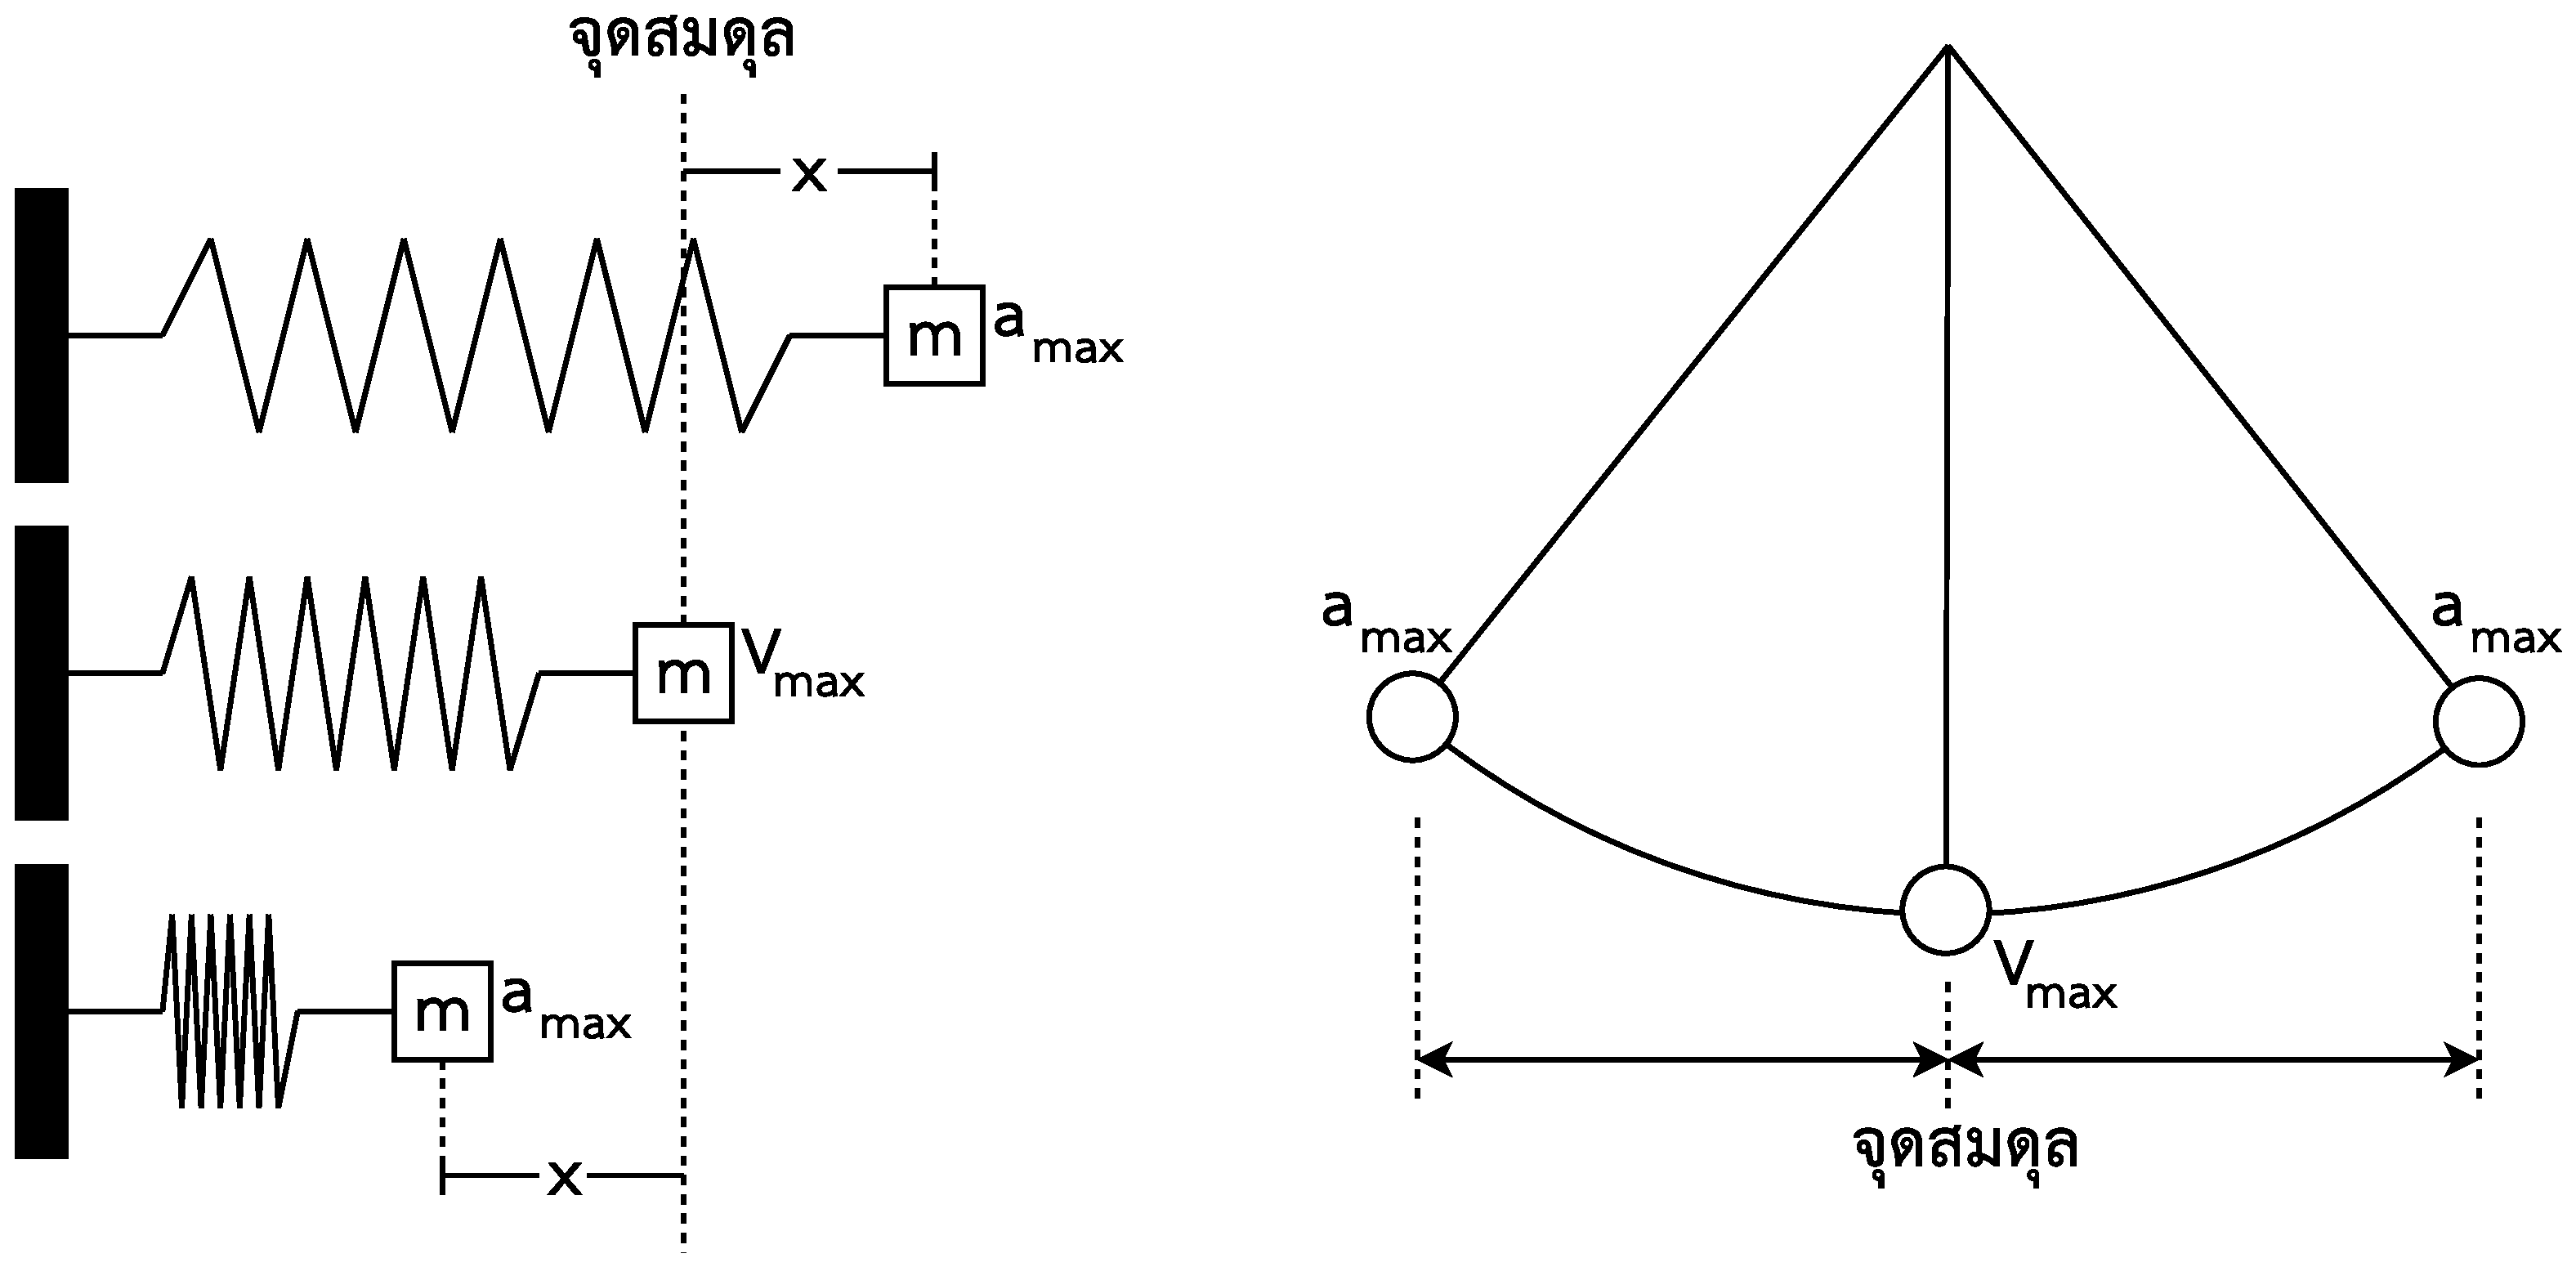
\includegraphics[width=\textwidth]{content-13.eps}
\end{center}
